\phantomsection

% Increment the chapter counter so \thechapter shows the correct number
% and make it referenceable with \ref
\refstepcounter{chapter}

% Manually add this appendix to the Table of Contents
\addcontentsline{toc}{chapter}{Apéndice \thechapter: Implementación del clúster virtualizado HTCondor}

% Add vertical space above the title (mimics standard chapter spacing)
\vspace{40pt}

% Display the actual chapter title (centered, large, bold)
{\centering \normalfont\huge\bfseries Apéndice~\thechapter: Implementación del clúster virtualizado HTCondor~\par}

% Add spacing between title and horizontal rule
\vspace{10pt}

% Draw a horizontal line across the page for visual separation
{\centering \rule{\textwidth}{0.4pt} \par}

% Add vertical space between title section and content
\vspace{40pt}

% Set the running headers for left and right pages
\markboth{Apéndice \thechapter: Implementación del clúster virtualizado HTCondor}{Apéndice \thechapter: Implementación del clúster virtualizado HTCondor}


\FloatBarrier\subsection{Instalación en un entorno virtualizado}

El clúster de computación distribuida de HTCondor actualmente soporta la versión \texttt{8.4.11}. A continuación se muestra la salida de uno de los nodos Raspberry-Pi, los cuales tienen una instalación heterogénea:

% HTCondor version output
\begin{minted}[
    frame=lines,
    framesep=2mm,
    baselinestretch=1.2,
    bgcolor=lightgray!10,
    fontsize=\footnotesize,
]{bash}
condor_version
$CondorVersion: 8.4.11 Feb 06 2017 BuildID: Debian-8.4.11~dfsg.1-1 Debian-8.4.11~dfsg.1-1
$$CondorPlatform: ARMV7L-Raspbian_ $
\end{minted}


Si bien esta versión es compatible con el \textbf{universo parallel}, la limitada documentación disponible para la version \texttt{8.4.11} en particular representó un obstáculo para implementar algoritmos que utilizaran OpenMPI. Por esta razón, y siguiendo la recomendación del asesor de este proyecto, se decidió implementar dicho universo en una infraestructura virtualizada.

\FloatBarrier\subsubsection{Infraestrutura virtualizada}

El primer paso hacia la implementación de la nueva infraestructura HTCondor fue desplegar máquinas virtuales en la infraestructura del \GRID. Para ello se utilizó un servidor dedicado que ejecuta el hipervisor \cite{xcpng_intro}, en el cual se configuraron 5 máquinas virtuales con el sistema operativo~\texttt{AlmaLinux 9.6 (Sage Margay) x86\_64}. Las máquinas pueden verse, mediante la interfaz Xen-Orchestra en la figura \ref{fig:xen-vms}. Esta configuración difiere significativamente de la arquitectura armv7l de 32 bits que utiliza el clúster de Raspberry Pi actual. La elección de este sistema operativo no fue trivial, se fundamentó en varios criterios: según la documentación oficial, AlmaLinux es uno de los sistemas operativos oficialmente soportados por HTCondor~\cite{HTCondor_install}, además de haber sido implementado exitosamente por instituciones como el CERN \citep{Bunsic2025}.

\begin{figure}
	\centering
	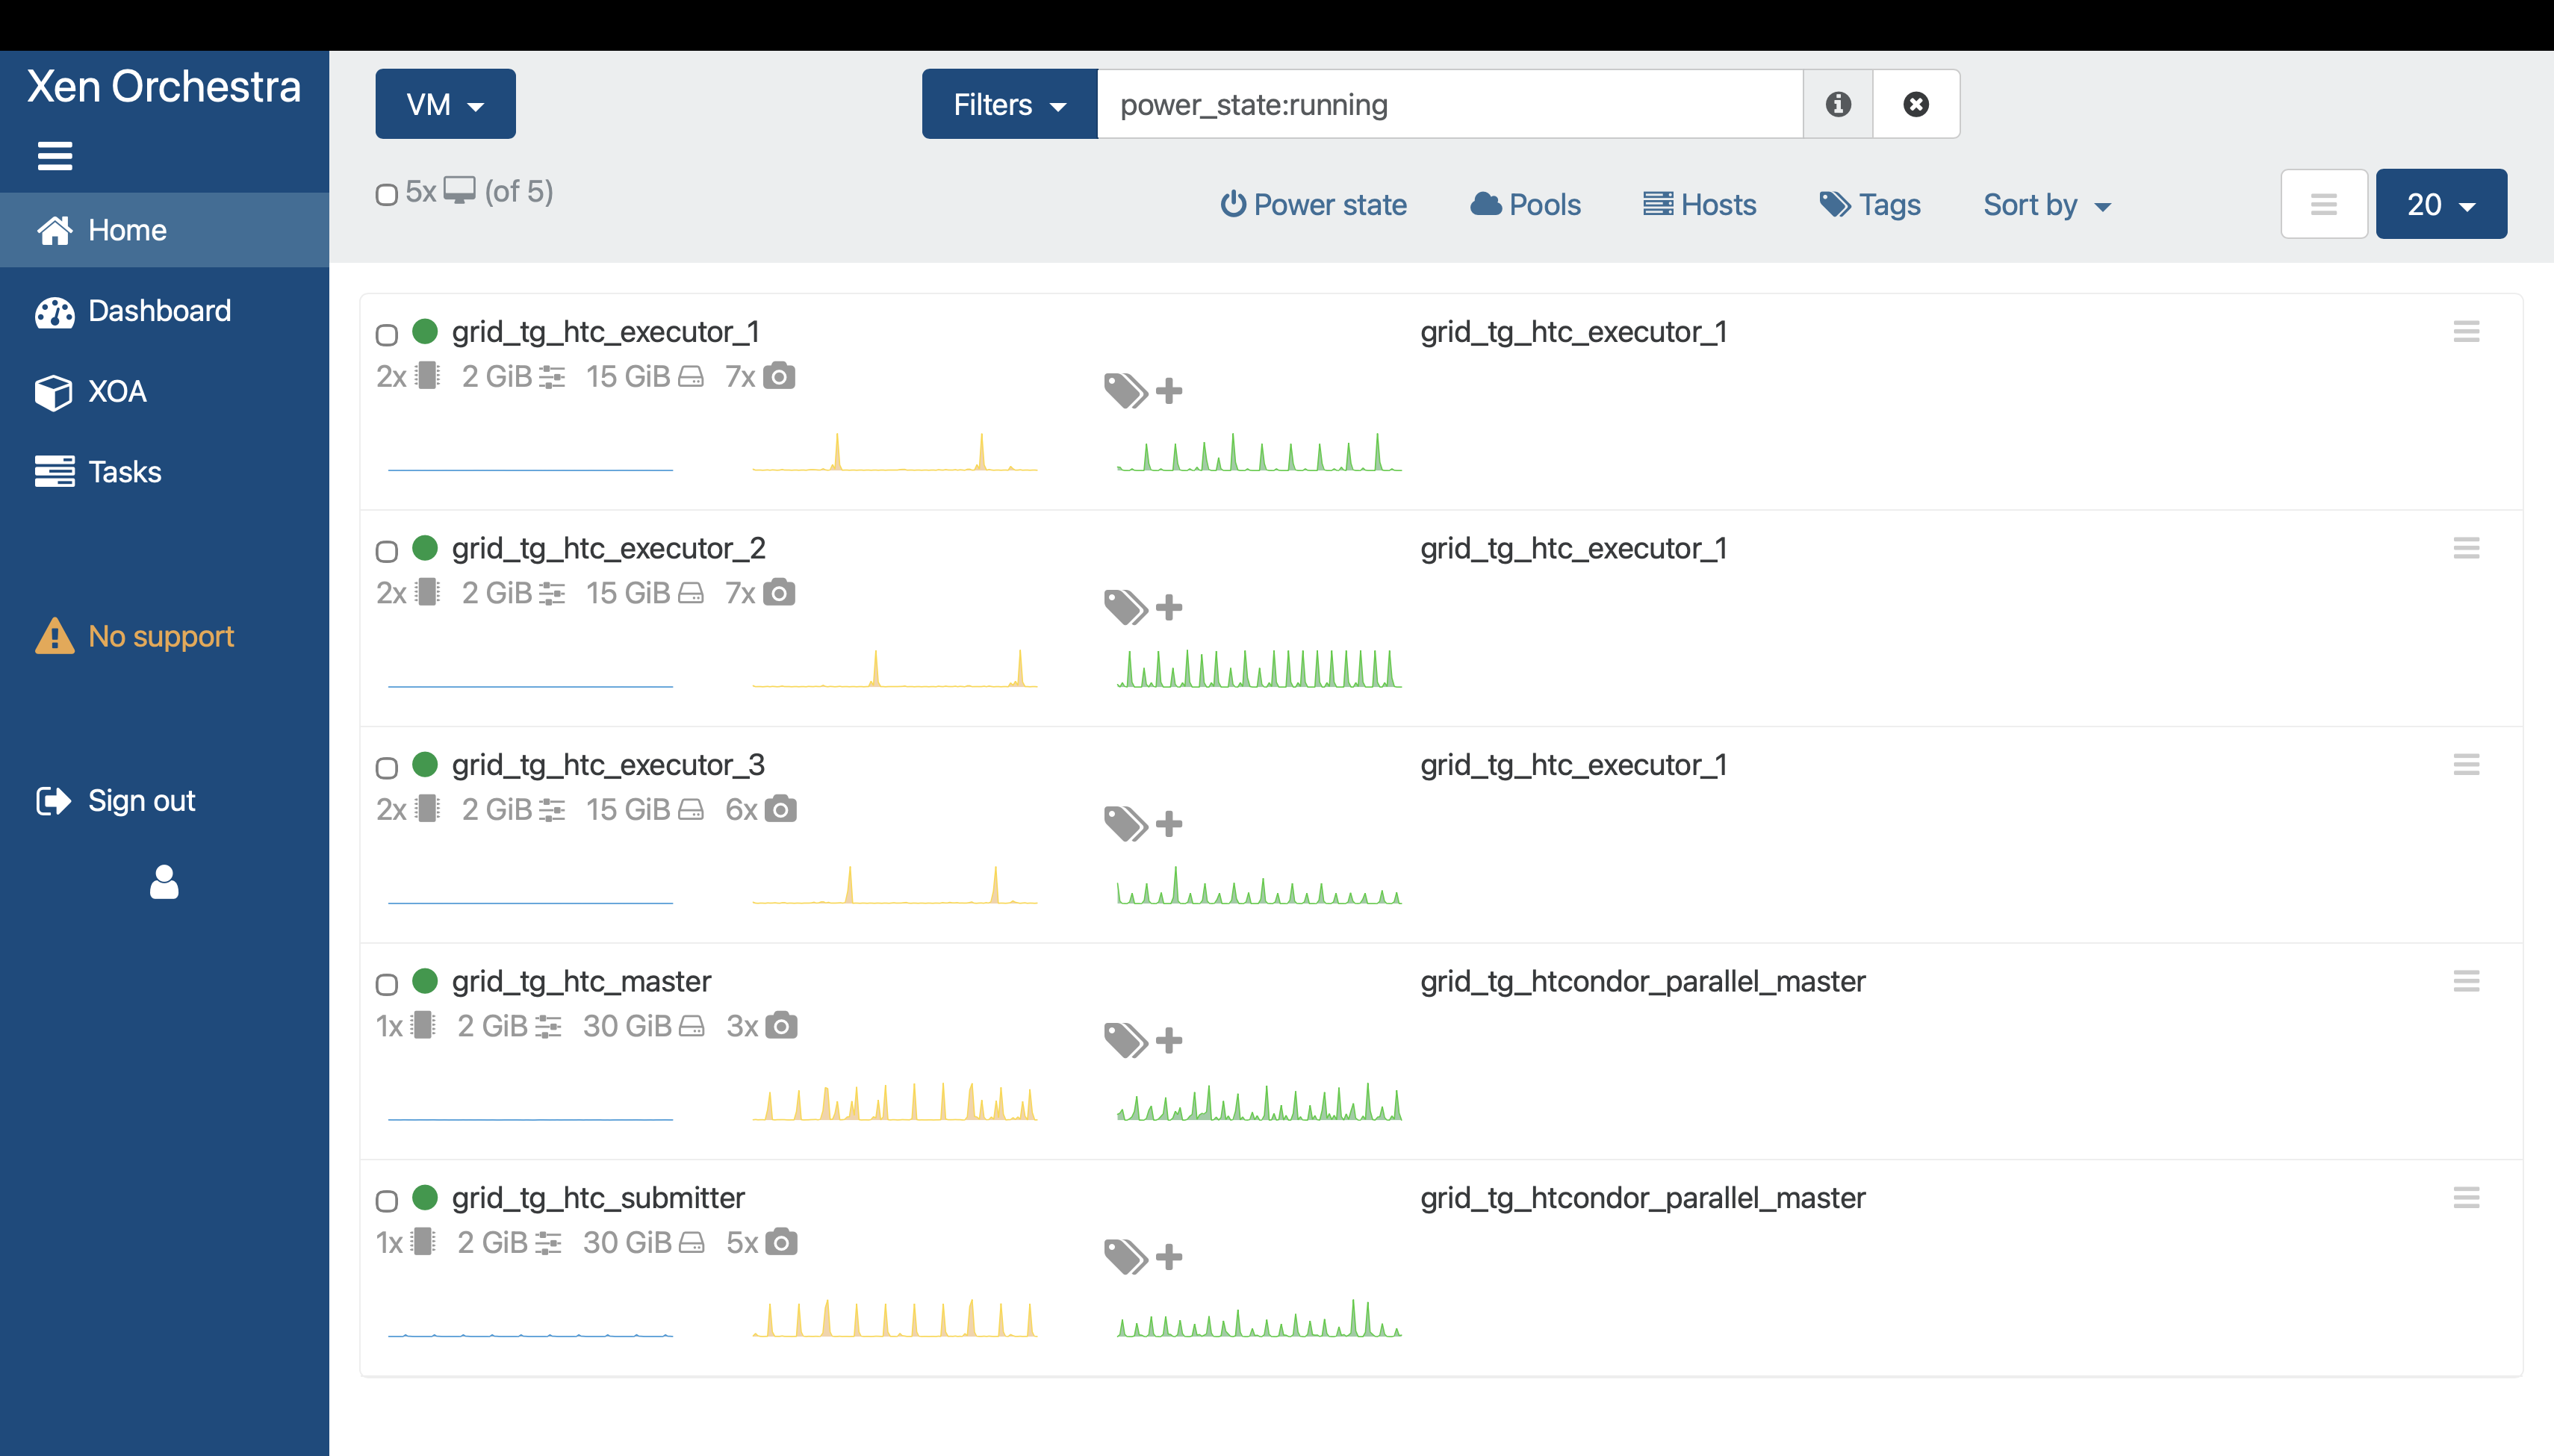
\includegraphics[scale=0.25]{apendices/infra-virtual/xen-vms.png}
	\caption{Vista de las máquinas virtuales para la nueva infraestructura HTCondor virtualizada de \GRID}
	\label{fig:xen-vms}
\end{figure}

A cada máquina se le asignó, al momento de instalación, una dirección IP dentro de la red \texttt{172.30.28.0/24} como se muestra en la Tabla~\ref{tab:nodos-htcondor}:

\begin{table}[H]
	\centering
	\renewcommand{\arraystretch}{1.2} % Espaciado reducido
	\fontsize{9pt}{10pt}\selectfont % Tamaño de fuente 9pt
	\begin{tabular}{|p{3cm}|p{3cm}|p{4.5cm}|p{2.5cm}|}  % Total: 14cm (incluyendo bordes)
		\hline
		\textbf{Rol del nodo} & \textbf{Dirección IP} & \textbf{Nombre de usuario} & \textbf{Usuario} \\ \hline
		Grid Manager          & 172.30.28.29          & gridmanager                & alma             \\ \hline
		Master                & 172.30.28.30          & master                     & alma             \\ \hline
		Submit                & 172.30.28.31          & submit                     & alma             \\ \hline
		Ejecutor 1            & 172.30.28.32          & exec01                     & alma             \\ \hline
		Ejecutor 2            & 172.30.28.33          & exec02                     & alma             \\ \hline
		Ejecutor 3            & 172.30.28.34          & exec03                     & alma             \\ \hline
	\end{tabular}
	\caption{Configuración de nodos del clúster HTCondor virtualizado}
	\label{tab:nodos-htcondor}
\end{table}


\FloatBarrier\subsubsection{Instalación de HTCondor}

Para la instalación de HTCondor se diseño el siguiente script, el cual emplea otro script que puede encontrarse en la documentación oficial \cite{HTCondor-linux-install}.



% HTCondor Install script
\begin{minted}[
    frame=lines,
    framesep=2mm,
    baselinestretch=1.2,
    bgcolor=lightgray!10,
    fontsize=\footnotesize,
]{bash}
#!/bin/bash

# Script de instalación de HTCondor para Alma Linux 9.6
# Uso: ./install-condor.sh <tipo_nodo> <hostname_master> <contraseña>
# Tipos de nodo: master, submit, worker

if [ "$#" -ne 3 ]; then
    echo "Uso: $0 <tipo_nodo> <hostname_master> <contraseña>"
    echo "Tipos de nodo: master, submit, worker"
    echo "Ejemplo: $0 master master.example.com micontraseña"
    exit 1
fi

NODE_TYPE=$1 #Tipo de nodo, hay tres opciones: {'master', 'submit' y 'worker;}
MASTER_FQN=$2 # Fully Qualified Name del nodo maestro.
PASSWORD=$3 #Deberá ser igual para todos los nodos de manera que puedan comunicarse entre sí

sudo dnf update -y

case $NODE_TYPE in
    master)
        echo "Instalando nodo MASTER..."
        curl -fsSL https://get.htcondor.org | sudo /bin/bash -s -- --no-dry-run --cm $MASTER_FQN --password $PASSWORD --channel lts
        ;;
    submit)
        echo "Instalando nodo SUBMIT (access point)..."
        curl -fsSL https://get.htcondor.org | sudo /bin/bash -s -- --no-dry-run --ap $MASTER_FQN --password $PASSWORD --channel lts
        ;;
    worker)
        echo "Instalando nodo WORKER (execution point)..."
        curl -fsSL https://get.htcondor.org | sudo /bin/bash -s -- --no-dry-run --ep $MASTER_FQN --password $PASSWORD --channel lts
        ;;
    *)
        echo "Error: Tipo de nodo inválido. Use: master, submit o worker"
        exit 1
        ;;
esac

echo "Instalación completada exitosamente!"
\end{minted}


Aparte del script anterior, también se creó una guía en formato .md la cual puede ser encontrada en el siguiente \href{https://github.com/Parritap/HTcondor/blob/master/alma-linux-cluster/README-ES.md}{https://github.com/Parritap/HTcondor/blob/master/alma-linux-cluster/README-ES.md}.



Para HTcondor es muy importante que los nodos puedan comunicarse entre sí, para lograr esto, se editaron los archivos \texttt{/etc/hosts} en cada uno de los nodos. Dicha edición puede verse en a continuación:

% HTCondor Install script
\begin{minted}[
    frame=lines,
    framesep=2mm,
    baselinestretch=1.2,
    bgcolor=lightgray!10,
    fontsize=\footnotesize,
]{bash}
#Parallel config
172.30.28.30 master
172.30.28.31 submit
172.30.28.32 exec01
172.30.28.33 exec02
172.30.28.34 exec03
172.30.28.35 exec04
\end{minted}

\FloatBarrier\subsection{Prueba de instalación exitosa}

Después de dicha configuración podremos ejecutar el comando \texttt{condor\_status} y ver lo siguiente impreso en consola, lo que indica que HTCondor encuentra a los nodos ejecutores dentro de la red, así como también que los nodos están publicando su disponibilidad dentro del clúster:

\begin{minted}[
    frame=lines,
    framesep=2mm,
    baselinestretch=1.2,
    bgcolor=lightgray!10,
    fontsize=\footnotesize,
]{bash}
Name         OpSys      Arch   State     Activity LoadAv Mem   ActvtyTime

slot1@exec01 LINUX      X86_64 Unclaimed Idle      0.000 1763  6+02:39:58
slot1@exec02 LINUX      X86_64 Unclaimed Idle      0.000 1763  6+02:34:51
slot1@exec03 LINUX      X86_64 Unclaimed Idle      0.000 1763  6+02:34:43

               Total Owner Claimed Unclaimed Matched Preempting  Drain Backfill BkIdle

  X86_64/LINUX     3     0       0         3       0          0      0        0      0

         Total     3     0       0         3       0          0      0        0      0
\end{minted}


\FloatBarrier\subsection{Instalación de un implementación \MPI}

Para permitir la comunicación entre trabajos distribuidos fuertemente acoplados en un pool HTCondor, es necesario implementar una tecnología basada en el estándar~\MPI. En este contexto, se seleccionó OpenMPI debido a que, según la documentación oficial de HTCondor \cite{HTCondor_Parallel}, esta implementación particular del estándar MPI cuenta con soporte nativo, lo que facilita su integración con el sistema de gestión de trabajos. Para el presente clúster se instaló la versión \texttt{4.1.5} la cuál se encuentra en la página oficial de \href{https://www.open-mpi.org/software/ompi/v4.1/}{OpenMPI}. El script de instalación de OpenMPI para el sistema operativo Alma Linux se presenta a continuación:

% HTCondor Install script
\begin{minted}[
    frame=lines,
    framesep=2mm,
    baselinestretch=1.2,
    bgcolor=lightgray!10,
    fontsize=\footnotesize,
]{bash}
# Debemos estar dentro de la carpeta que contiene el archivo producto de 
# descomprimir el archibo .tar de openmpi (disnponible en su página oficial)
# en nuestro caso el archivo tar fue openmpi-4.1.5.tar.gz para todas las máquinas

sudo dnf update -y
dnf install -y gcc gcc-c++ gcc-gfortran make libtool m4 automake wget tar
sudo dnf groupinstall "Development Tools" -y
./configure --prefix=/opt/openmpi
make -j$(nproc)
sudo make install
\end{minted}


\FloatBarrier\subsection{Configurción de OpenMPI en HTCondor}

El primer paso consiste en crear un archivo de configuración en el que se defina el \textbf{Scheduler dedicado} para los nodos ejecutores. Además, es necesario establecer parámetros que permitan a estos nodos priorizar los trabajos dedicados y evitar la suspensión de tareas enviadas. Según la documentación oficial de HTCondor \cite{HTCondor_Parallel}, se recomienda reservar un conjunto de máquinas exclusivas para el universo parallel. En este clúster, esta configuración se implementó en el archivo \texttt{/etc/condor/config.d/50-parallel.config} de cada nodo ejecutor, cuyo contenido se muestra a continuación:


% HTCondor 50-parallel.config file
\begin{minted}[
    frame=lines,
    framesep=2mm,
    baselinestretch=1.2,
    bgcolor=lightgray!10,
    fontsize=\footnotesize,
]{bash}
DedicatedScheduler = "DedicatedScheduler@submit"
STARTD_ATTRS = $(STARTD_ATTRS), DedicatedScheduler
##-------------------------------------------------------------------
## 2) Always run jobs, but prefer dedicated ones
##--------------------------------------------------------------------
START          = True
SUSPEND        = False
CONTINUE       = True
PREEMPT        = False
KILL           = False
WANT_SUSPEND   = False
WANT_VACATE    = False
RANK = Scheduler =?= $(DedicatedScheduler) 
##--------------------------------------------------------------------
MPI_CONDOR_RSH_PATH = $(LIBEXEC)
CONDOR_SSHD = /usr/sbin/sshd
CONDOR_SSH_KEYGEN = /usr/bin/ssh-keygen
OPENMPI_INSTALL_PATH = /opt/openmpi/bin/ # Lugar común donde se está instalado OpenMPI en los nodos workers
MOUNT_UNDER_SCRATCH = /tpm
\end{minted}

También es necesario especificar en la máquina submit la ubicación donde está instalado OpenMPI en los nodos ejecutores. En este caso, la configuración correspondiente se encuentra en el archivo \texttt{/etc/condor/02-openmpi.config}. El contenido de este archivo se muestra a continuación:

% HTCondor submit  02-openmpi.config file
\begin{minted}[
    frame=lines,
    framesep=2mm,
    baselinestretch=1.2,
    bgcolor=lightgray!10,
    fontsize=\footnotesize,
]{bash}
OPENMPI_INSTALL_PATH = /opt/openmpi
MOUNT_UNDER_SCRATCH = /tmp
\end{minted}

